\documentclass[aspectratio=169,11pt,t]{beamer}
% ============================================================
%  ksa-cs-v2: ksa-cs-lecture-template.tex 스타일 + 한글, v2 덱(16:9)용.
%    - 짙은 네이비 헤드라인 (섹션 이름 + 프레임마다 점)
%    - 꽉 찬 파란 제목 막대, 둥근 그림자 블록
%    - 한글: Noto Sans CJK KR (fontspec)
%  사용:
%    \documentclass[aspectratio=169,11pt,t]{beamer}
%    \input{<..>/theme/ksa-cs-v2.tex}
%  ksa-theme.tex 의 매크로(\kb \kq, ksablue/ksared 등)도 같은 이름으로 둔다
%  -> v2 덱 본문을 거의 그대로 옮길 수 있다.
% ============================================================

\usepackage{fontspec}
\usepackage{amsmath,amssymb}
\usepackage{tikz}
\usepackage{listings}
\usepackage{graphicx}
\usepackage{booktabs}
\usepackage{varwidth}
% enumitem 은 넣지 않는다 (beamer 글머리표가 사라진다)

\defaultfontfeatures{Ligatures=TeX}
\setmainfont{Noto Sans CJK KR}
\setsansfont{Noto Sans CJK KR}
\setmonofont{Noto Sans Mono CJK KR}[Scale=0.92]
\usefonttheme{professionalfonts}

% ---------- 기본 틀 ----------
\usetheme{default}
\useinnertheme[shadow=true]{rounded}
\setbeamertemplate{navigation symbols}{}
\setbeamersize{text margin left=1em,text margin right=1em}

% ---------- 색 (템플릿 원본 값) ----------
\definecolor{navydark}{HTML}{191959}
\definecolor{navydim}{HTML}{8888B0}
\definecolor{navytitle}{HTML}{262686}
\definecolor{navyblue}{HTML}{3333B2}
\definecolor{blockbodybg}{HTML}{E9E9F3}
\definecolor{examplegreen}{HTML}{006000}
\definecolor{examplebg}{HTML}{E5EFE5}
\definecolor{alertred}{HTML}{BF0000}
\definecolor{alertbg}{HTML}{F9E5E5}
% ksa-theme.tex 와 같은 이름 (본문 호환)
\colorlet{ksablue}{navytitle}
\colorlet{ksabluedk}{navydark}
\definecolor{ksagold}{HTML}{D6CBB1}
\definecolor{ksagolddk}{HTML}{A9976B}
\colorlet{ksared}{alertred}
\definecolor{ksagray}{HTML}{5B5B5B}

\setbeamercolor{structure}{fg=navyblue}
\setbeamercolor{alerted text}{fg=alertred}
\setbeamercolor{frametitle}{bg=navytitle,fg=white}
\setbeamercolor{title}{fg=white,bg=navytitle}
\setbeamercolor{block title}{bg=navytitle,fg=white}
\setbeamercolor{block body}{bg=blockbodybg,fg=black}
\setbeamercolor{block title example}{bg=examplegreen,fg=white}
\setbeamercolor{block body example}{bg=examplebg,fg=black}
\setbeamercolor{block title alerted}{bg=alertred,fg=white}
\setbeamercolor{block body alerted}{bg=alertbg,fg=black}
\setbeamercolor{item}{fg=navyblue}
\setbeamertemplate{itemize item}[circle]
\setbeamertemplate{itemize subitem}[triangle]

% ---------- 헤드라인: miniframes (섹션 이름 + 점) ----------
\useoutertheme[subsection=false]{miniframes}
\setbeamerfont{section in head/foot}{size=\tiny}
\setbeamercolor{section in head/foot}{bg=navydark,fg=white}
\setbeamercolor{mini frame}{fg=white}
\setbeamertemplate{mini frames}[circle]

% ---------- 제목 막대: 폭 꽉 채움, 두 줄까지 ----------
\setbeamerfont{frametitle}{size=\normalsize,series=\bfseries}
\setbeamertemplate{frametitle}{%
  \nointerlineskip
  \begin{beamercolorbox}[wd=\paperwidth,ht=2.7ex,dp=1.1ex,leftskip=.3cm,rightskip=.3cm]{frametitle}%
    \usebeamerfont{frametitle}\insertframetitle
  \end{beamercolorbox}}

% ---------- 쪽 번호: 오른쪽 아래 ----------
\setbeamertemplate{footline}{%
  \hfill
  {\color{navydim}\scriptsize\insertframenumber\,/\,\inserttotalframenumber}%
  \hspace{3mm}\vspace{2mm}%
}

% ---------- 표지: 템플릿처럼 헤드라인은 그대로, 가운데 둥근 그림자 상자에 제목 한 줄 ----------
% 덱에서:  {\setbeamertemplate{footline}{}\begin{frame}[c,noframenumbering]\titlepage\end{frame}}
\setbeamercolor{title}{fg=white,bg=navyblue}
\makeatletter
\setbeamertemplate{title page}{%
  \vfill
  \centering
  \begin{minipage}{0.84\paperwidth}
  \begin{beamercolorbox}[wd=\linewidth,sep=7pt,center,rounded=true,shadow=true]{title}
    {\usebeamerfont{title}\inserttitle\par}%
    \ifx\insertsubtitle\@empty\else\vskip0.4em{\usebeamerfont{subtitle}\insertsubtitle\par}\fi
  \end{beamercolorbox}
  \end{minipage}\par\vskip1.6em
  {\usebeamerfont{author}\color{navytitle}\insertauthor\par}\vskip0.3em
  {\usebeamerfont{institute}\color{ksagray}\insertinstitute\par}
  \vfill
}
\makeatother
\setbeamerfont{title}{series=\bfseries,size=\Large}
\setbeamerfont{subtitle}{size=\normalsize}
\setbeamerfont{author}{size=\normalsize}
\setbeamerfont{institute}{size=\small}

% ksa-theme 호환: 덱이 \renewcommand{\ksacredit}{..} 를 해도 되게 (꼬리말에는 안 쓴다)
\newcommand{\ksacredit}{}

% ---------- 강조 ----------
\newcommand{\hl}[1]{\textcolor{alertred}{#1}}
\newcommand{\hlb}[1]{\textcolor{navyblue}{#1}}
\newcommand{\kb}[1]{\textbf{\color{ksablue}#1}}
\newcommand{\kq}[1]{\textbf{\color{ksared}#1}}

% ---------- 파이썬 코드 (템플릿과 같은 색) ----------
\definecolor{codekw}{HTML}{0033B3}
\definecolor{codebuiltin}{HTML}{BF0000}
\definecolor{codestr}{HTML}{067D17}
\definecolor{codecomment}{HTML}{8C8C8C}
\definecolor{codenum}{HTML}{1750EB}
\lstdefinestyle{py}{
  language=Python, basicstyle=\ttfamily\scriptsize,
  keywordstyle=\color{codekw}\bfseries, stringstyle=\color{codestr},
  commentstyle=\color{codecomment}\itshape, numberstyle=\color{codenum},
  emph={print,len,range,sum,input,int,str,float,list,dict,append,remove,sorted,abs,min,max},
  emphstyle=\color{codebuiltin}, showstringspaces=false, keepspaces=true,
  columns=fixed, basewidth=0.52em, aboveskip=1mm, belowskip=1mm, xleftmargin=2mm,
  breaklines=true
}
\lstset{style=py}

% 원본 덱 (ksa-theme): slides/v2/ml1/week02/logistic_regression/ -- 그림은 거기 figs/ 를 그대로 쓴다
\setbeamerfont{author}{size=\normalsize}
\setbeamerfont{institute}{size=\small}
\graphicspath{{figs/}{../../../v2/ml1/week02/logistic_regression/figs/}{../../../assets/}}
\makeatletter
\newcommand{\markpage}[1]{\protected@write\@auxout{}{\string\newlabel{#1}{{\the\c@framenumber}{}}}\hypertarget{#1}{}}
\newcommand{\pref}[1]{\hyperlink{#1}{\textcolor{ksagolddk}{(p.\ref{#1})}}}
\makeatother

\renewcommand{\ksacredit}{Machine Learning and Deep Learning \,\textperiodcentered\, 로지스틱회귀}
\title{로지스틱회귀 (Logistic Regression)}
\subtitle{숫자 대신 확률을 예측하기}
\author{Machine Learning and Deep Learning}
\institute{한국과학영재학교 (KSA)}
\date{}
\begin{document}
{\setbeamertemplate{footline}{}\begin{frame}[c,noframenumbering]\titlepage\end{frame}}

\section{질문}
% --- lichess 대국 화면
\begin{frame}{lichess 한 판: 이름 옆 숫자가 레이팅}
\vfill
\centering
\begin{tikzpicture}
\node[anchor=south west,inner sep=0] (img) at (0,0) {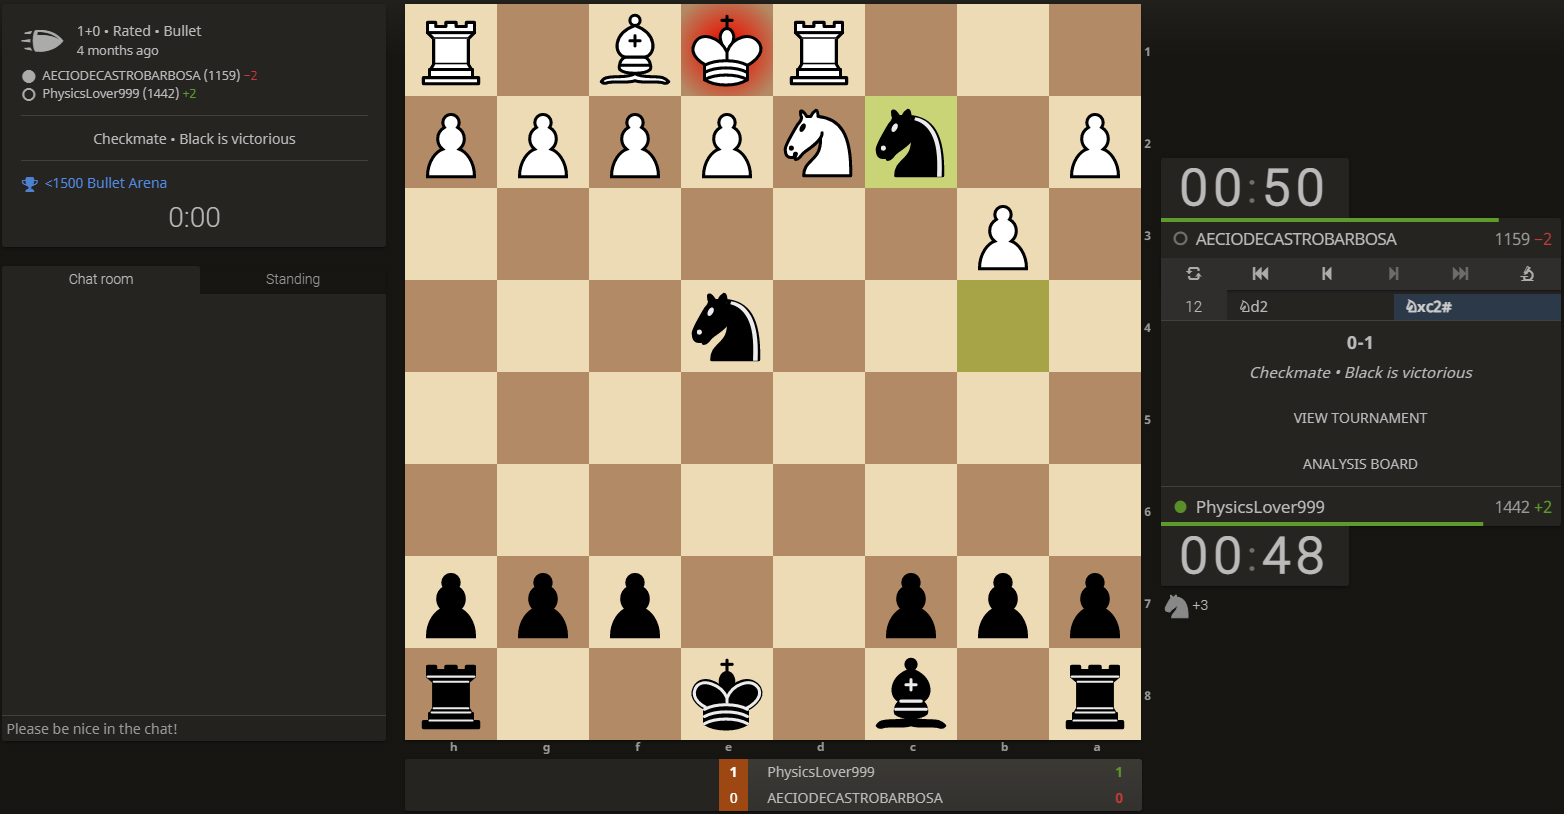
\includegraphics[width=0.74\linewidth]{pasted_p2_5493f117.png}};
\begin{scope}[x={(img.south east)},y={(img.north west)}]
\draw[red,ultra thick,rounded corners=2pt] (0.945,0.680) rectangle (1.0,0.732);
\draw[red,ultra thick,rounded corners=2pt] (0.945,0.352) rectangle (1.0,0.404);
\end{scope}
\end{tikzpicture}\par\vskip0.3em
{\large 백 \kb{1159} 대 흑 \kb{1442}: 283점 높은 흑이 이겼다}
\vfill
\note{lichess에서 실제로 둔 1분 불릿 한 판입니다. 이름 옆 빨간 상자 안의 숫자가 레이팅, 실력 점수입니다. 백은 1159점, 흑은 1442점으로 흑이 283점 높았고, 결과도 흑이 체크메이트로 이겼습니다. 그러면 레이팅이 몇 점 높으면 몇 퍼센트쯤 이길까요? 이게 오늘의 질문입니다.}
\end{frame}

% --- 오늘의 질문
\begin{frame}{오늘의 질문: 레이팅이 200점 높으면 몇 \% 이길까?}
\vfill
\centering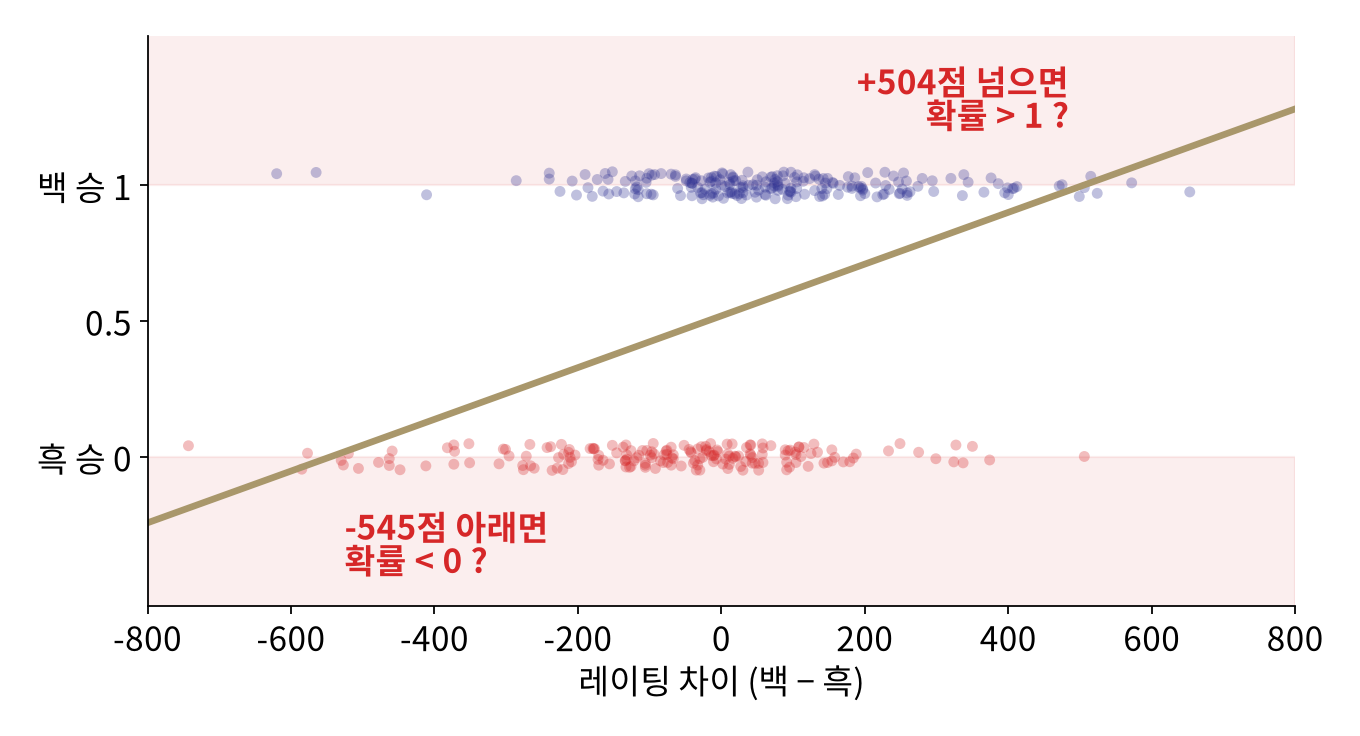
\includegraphics[width=0.54\linewidth]{chess_line.png}\par\vskip0.2em
{\large 백 한 사람 기준으로: 레이팅 차이로 \kb{이기면 1, 지면 0}을 예측: 직선을 그으면?}\\[0.2em]
{\small 온라인 체스 lichess, 2013년 1월 승패가 난 117,003판 중 400판 표시 \quad 레이팅 = 게임 랭크 점수 (MMR) 와 같은 것}\\[0.1em]
{\small 백 · 흑은 레이팅과 상관없이 정해진다: 백이 더 높은 판 52\%, 흑이 더 높은 판 48\% (앞 쪽처럼 $x < 0$)}
\vfill
\note{온라인 체스 사이트 lichess의 실제 대국 약 12만 판입니다. 게임의 랭크 점수, MMR처럼 체스에도 실력 점수인 레이팅이 있습니다. 가로축은 백의 레이팅에서 흑의 레이팅을 뺀 차이, 세로축은 백이 이겼으면 1, 졌으면 0입니다. 백 한 사람의 입장에서만 보는 겁니다. 백과 흑은 레이팅과 상관없이 정해져서, 백이 더 높은 판이 52퍼센트, 앞 쪽의 판처럼 흑이 더 높은 판이 48퍼센트입니다. 가로축이 음수인 왼쪽이 백이 더 약한 판입니다. 레이팅이 높은 쪽 기준으로 보면 차이가 늘 플러스라 그래프의 절반만 남고, 뒤에서 볼 먼저 두는 쪽의 이점도 볼 수 없어서 백 기준으로 둡니다. 무승부는 뺐습니다. 지난 시간의 선형회귀처럼 직선을 그어 보면 어떨까요? 백이 504점 넘게 높으면 직선이 1을 넘어 확률이 100퍼센트보다 커지고, 545점 넘게 낮으면 0보다 작아집니다. 확률로 읽을 수가 없습니다.}
\end{frame}

% --- 구간별 비율
\begin{frame}{점을 세어 보면: 비율은 S 자}
\markpage{rate}
\vfill
\centering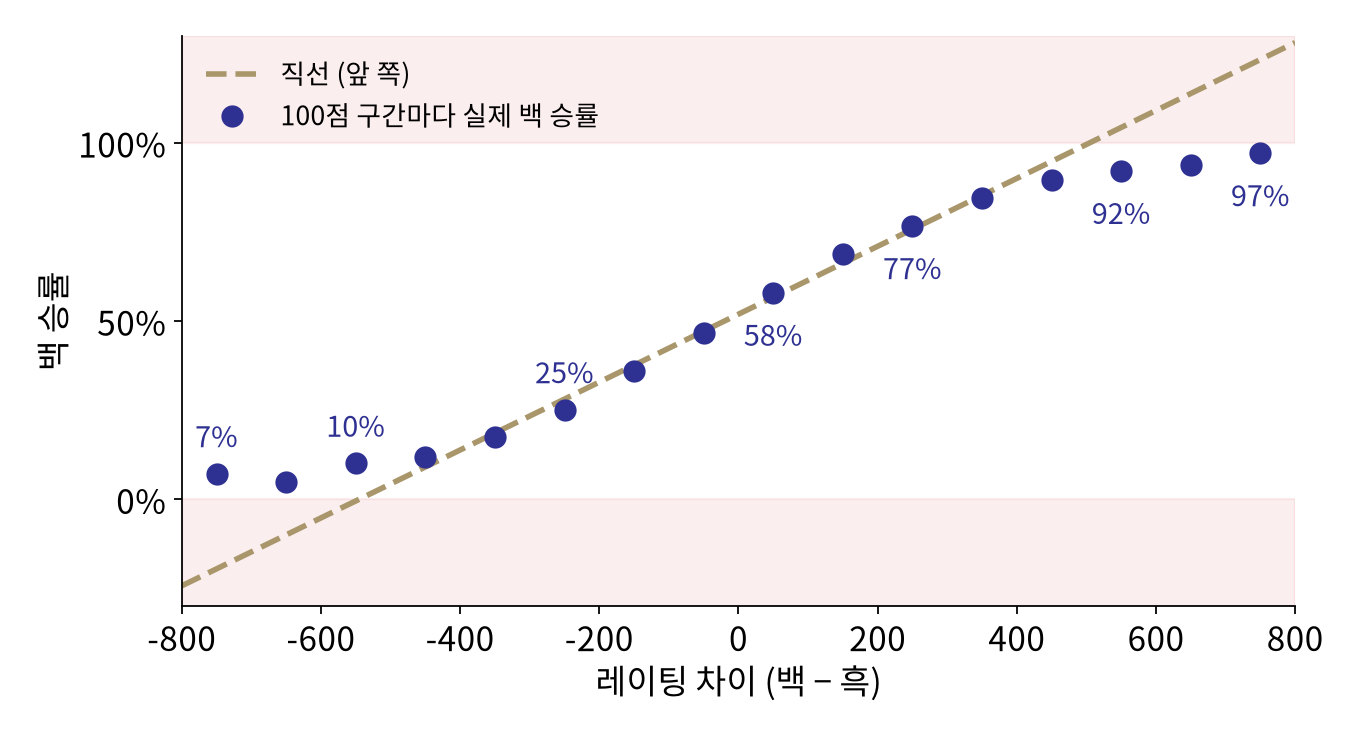
\includegraphics[width=0.54\linewidth]{chess_rate.png}\par\vskip0.2em
{\large 100점 구간마다 백 승률: $-500$ 점이면 10\%, 비슷하면 반반, $+500$ 점이면 92\%}\\[0.3em]
{\large 예측할 것은 0 / 1 이 아니라 \kb{이 비율 = 확률} \quad 0 과 1 사이에서 \kb{S 자}로 눕는다}\\[0.2em]
{\small 차이가 클수록 승률이 오르지만, 아무리 강해도 100\% 는 못 넘는다: 직선은 끝에서 빗나간다}
\vfill
\note{점 하나하나는 0 아니면 1이라 패턴이 잘 안 보입니다. 그래서 레이팅 차이 100점 구간마다 백이 몇 퍼센트 이겼는지 세어 봤습니다. 백이 500점 낮으면 10퍼센트, 비슷하면 반반, 500점 높으면 92퍼센트를 이깁니다. 차이가 클수록 승률이 오르지만, 아무리 실력 차이가 커도 100퍼센트를 넘을 수는 없으니 양 끝에서 눕습니다. 그래서 비율은 S 자입니다. 우리가 예측할 것은 0이나 1이 아니라 바로 이 비율, 확률입니다. 가운데에서는 직선도 괜찮지만, 끝으로 가면 직선은 0과 1 밖으로 빗나갑니다. 그러면 S 자 곡선을 쓰면 되겠죠.}
\end{frame}

\section{모델}
% --- 시그모이드
\begin{frame}{시그모이드: 아무 수나 0과 1 사이로}
\markpage{sigmoid}
\vfill
\begin{columns}[c]
\begin{column}{0.55\textwidth}\centering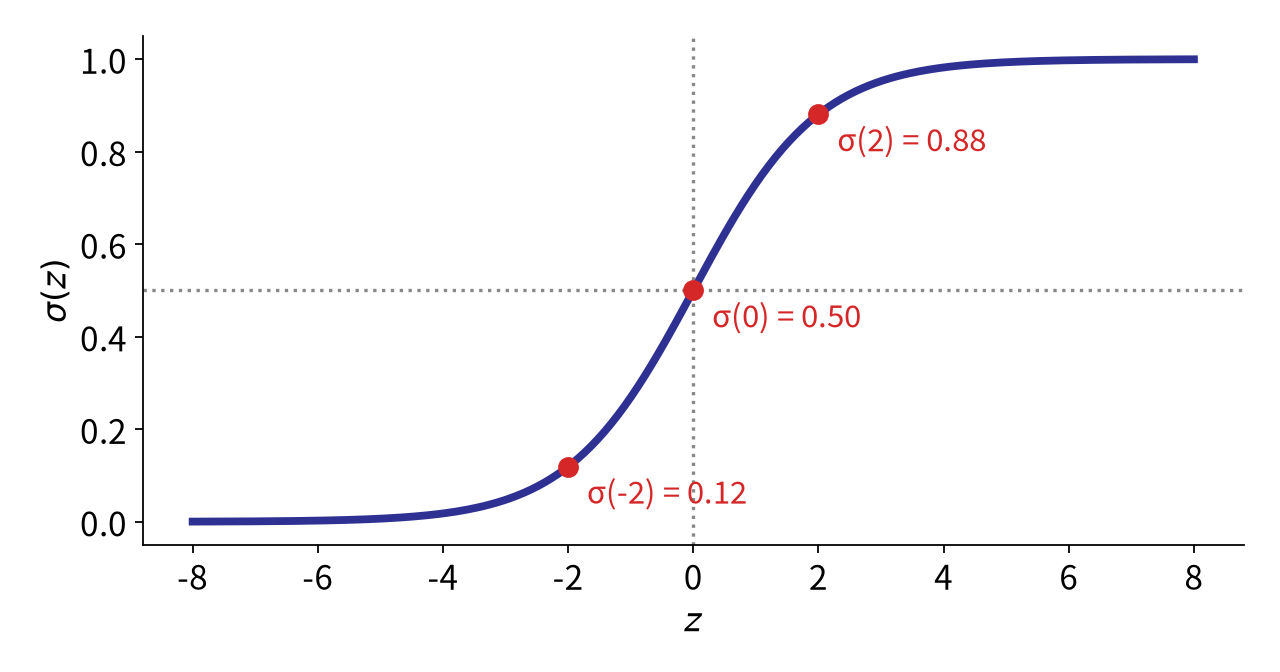
\includegraphics[width=\linewidth]{logit_sigmoid.png}\end{column}
\begin{column}{0.42\textwidth}
{\LARGE\[ \sigma(z) = \frac{1}{1 + e^{-z}} \]}\vskip0.4em
$z$ 가 크면 $\to 1$, \quad $z$ 가 작으면 $\to 0$\\[0.3em]
$z = 0$ 이면 정확히 $0.5$
\end{column}
\end{columns}
\vfill
\note{그래서 직선의 값을 시그모이드라는 함수에 한 번 통과시킵니다. 시그모이드는 어떤 수를 넣어도 0과 1 사이 값을 내놓습니다. 큰 수를 넣으면 1에 가까워지고, 작은 수를 넣으면 0에 가까워지고, 0을 넣으면 정확히 0.5가 나옵니다. 2를 넣으면 0.88, 마이너스 2를 넣으면 0.12입니다.}
\end{frame}

% --- 모델
\begin{frame}{로지스틱회귀 모델}
\vfill
\centering
{\LARGE\[ \hat y = \sigma(\underbrace{w_0 + w_1 x}_{z}) = P(\text{white wins} \mid x) \]}\vskip0.6em
{\large 선형회귀의 직선 $z$ 를 그대로 쓰고, 마지막에 $\sigma$ 만 씌운다 \quad $\to$ S 자 곡선}\\[0.6em]
{\large $x$ = 레이팅 차이 (백 $-$ 흑) \quad 출력 $\hat y$ = \kb{백이 이길 확률}}\\[0.4em]
{\small 이름은 ``회귀''지만 하는 일은 \kb{분류} \quad 수식에서는 백 승을 `white wins' 로 쓴다}
\vfill
\note{로지스틱회귀는 선형회귀의 직선 z를 그대로 계산하고, 마지막에 시그모이드만 씌운 모델입니다. 직선을 시그모이드에 넣으니 결과가 S 자 곡선이 되고, 0과 1 밖으로 나가지 않습니다. 입력 x는 레이팅 차이, 출력 와이햇은 백이 이길 확률로 읽습니다. 이름에 회귀가 들어가 있지만, 확률을 보고 누가 이길지 나누니까 실제로 하는 일은 분류입니다.}
\end{frame}

% --- 학습 결과
\begin{frame}{12만 판으로 학습하면}
\markpage{fit}
\vfill
\centering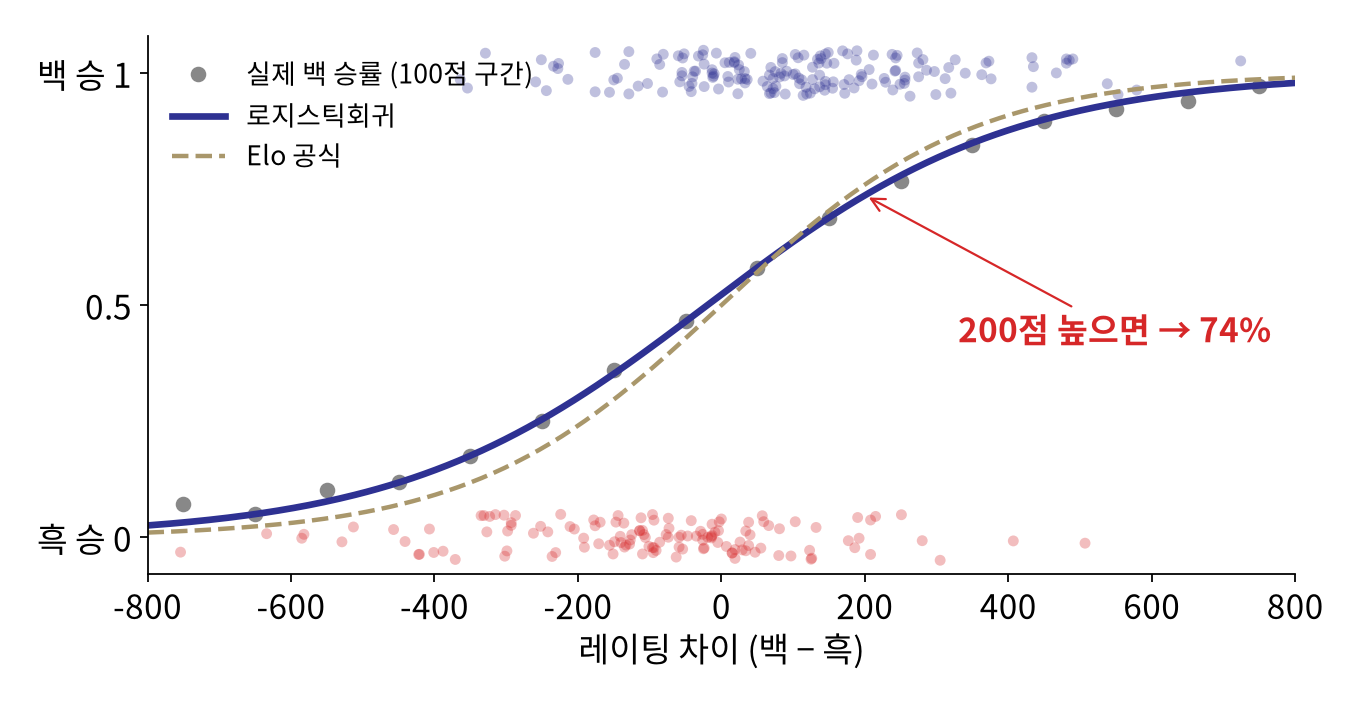
\includegraphics[width=0.6\linewidth]{chess_fit.png}\par\vskip0.3em
{\large $\hat y = \sigma(0.09 + 0.0047\,x)$ \qquad \kq{백이 200점 높으면 $\to$ 백 승률 74\%}}\\[0.2em]
{\small 레이팅을 정하는 \textbf{Elo 공식} $\frac{1}{1 + 10^{-x/400}} = \sigma(0.0058\,x)$ 도 같은 꼴: 레이팅 시스템이 곧 로지스틱회귀}
\vfill
\note{12만 판으로 학습하면 w0는 0.09, w1은 0.0047이 나옵니다. 파란 곡선이 레이팅 차이에 따른 백 승률이고, 회색 점은 앞에서 센 구간별 실제 비율입니다. 숫자 두 개짜리 곡선이 12만 판의 비율을 거의 그대로 따라갑니다. 200점 높으면 74퍼센트를 이깁니다. 재미있는 건 노란 점선입니다. 체스의 레이팅을 계산하는 Elo 공식은 1 나누기 1 더하기 10의 마이너스 x 나누기 400제곱인데, 이걸 정리하면 시그모이드 0.0058 x, 바로 로지스틱 곡선입니다. 체스, 바둑, 게임 랭크 점수는 처음부터 로지스틱회귀의 모양으로 설계된 겁니다. 데이터에서 배운 기울기 0.0047이 공식의 0.0058과 비슷하게 나왔습니다.}
\end{frame}

\section{결정 경계}
% --- 결정 경계
\begin{frame}{결정 경계: $z = 0$ 인 곳}
\vfill
\centering
{\Large\[ \hat y \ge 0.5 \;\Longleftrightarrow\; z = w_0 + w_1 x \ge 0 \;\Longleftrightarrow\; x \ge -\frac{w_0}{w_1} = -\frac{0.09}{0.0047} \approx -20 \]}\vskip0.8em
{\large 백은 \kb{20점 약해도} 반반: 먼저 두는 쪽이 유리하다 \quad (레이팅이 같으면 $\sigma(0.09) \approx$ \kb{52\%})}\\[0.5em]
{\large 시그모이드는 $z=0$ 에서 0.5 \pref{sigmoid} $\to$ \kb{경계는 직선 $z = 0$ 이 정한다}}\\[0.5em]
{\small 절편 $w_0$ 에도 뜻이 있다: 실력이 같을 때의 백의 이점}
\vfill
\note{확률이 0.5 이상이면 백 승이라고 판정할 때, 그 경계가 어디인지 식으로 구해 봅시다. 시그모이드는 z가 0일 때 0.5니까, 와이햇이 0.5 이상인 것은 z가 0 이상인 것과 같습니다. z는 w0 더하기 w1 x이니까 x가 마이너스 0.09 나누기 0.0047, 약 마이너스 20점 이상이면 됩니다. 백은 20점 약해도 반반이라는 뜻입니다. 체스는 백이 먼저 두니까 조금 유리하죠. 레이팅이 같을 때 백의 승률은 시그모이드 0.09, 약 52퍼센트입니다. 이렇게 절편 w0에도 뜻이 있습니다.}
\end{frame}

% --- 두 특징
\begin{frame}{특징이 둘이면: 경계는 직선}
\vfill
\begin{columns}[c]
\column{0.44\linewidth}\centering
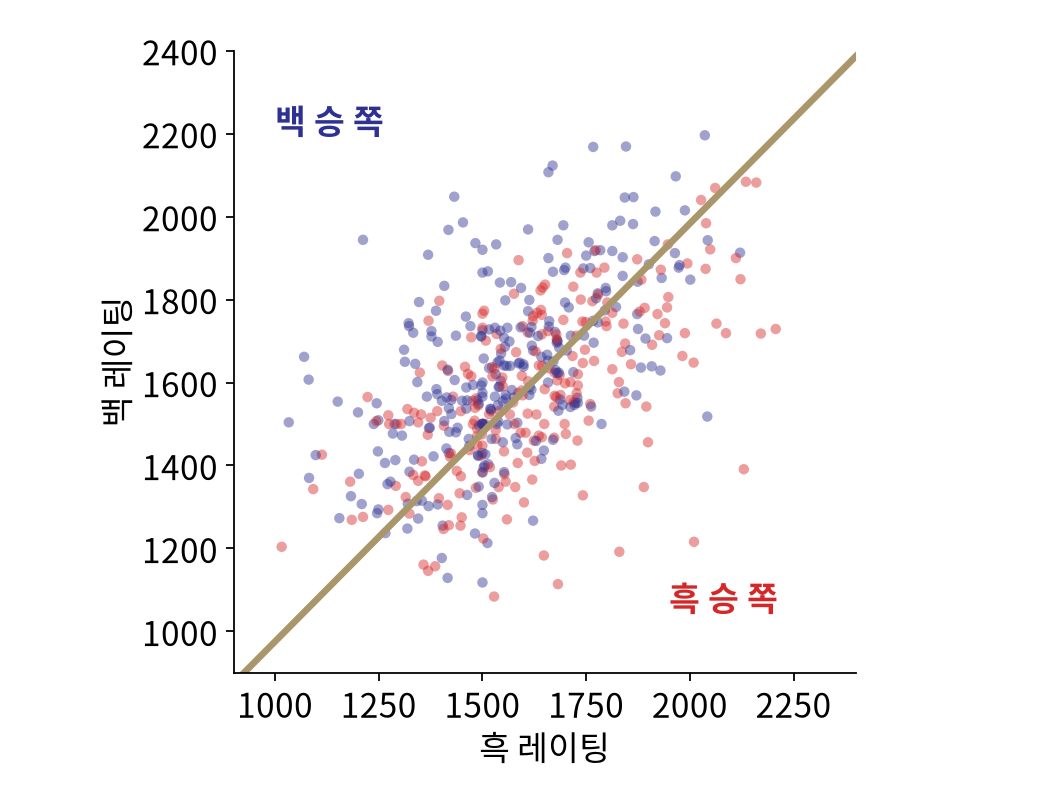
\includegraphics[width=\linewidth]{chess_2d.png}
\column{0.54\linewidth}
{\large 특징을 백 레이팅 $a$, 흑 레이팅 $b$ 따로 넣으면}\\[0.3em]
{\large $z = 0.15 + 0.00466\,a - 0.00470\,b$}\\[0.8em]
{\large 경계 $z = 0$ 은 평면 위의 \kb{직선} \quad $a \approx b - 32$}\\[0.3em]
{\large 두 계수가 \kb{크기는 같고 부호만 반대}}\\[0.2em]
{\large $\to$ 모델이 스스로 ``\textbf{차이}만 중요하다''를 찾았다}\\[0.6em]
{\small 1,000 점끼리든 2,000 점끼리든 차이가 같으면 승률도 같다 (Elo 의 생각)}
\end{columns}
\vfill
\note{특징이 두 개면 어떨까요? 이번에는 차이를 미리 빼지 않고, 백 레이팅 a와 흑 레이팅 b를 따로 넣어 봅니다. 파란 점이 백 승, 빨간 점이 흑 승입니다. 학습하면 z는 0.15 더하기 0.00466 a 빼기 0.00470 b이고, z가 0인 곳이 경계니까 평면 위의 직선, 거의 a가 b 빼기 32인 대각선입니다. 두 계수가 크기는 거의 같고 부호만 반대입니다. 따로 넣어 줬는데도 모델이 스스로 둘의 차이만 중요하다는 걸 찾아낸 겁니다. 1000점끼리 두든 2000점끼리 두든, 차이가 같으면 승률이 같다. 이게 Elo 레이팅의 생각입니다. 특징이 더 많아지면 경계는 평면, 초평면이 되지만 여전히 곧습니다. 그래서 로지스틱회귀를 선형 분류기라고 부릅니다.}
\end{frame}

% --- 오즈
\begin{frame}{$w_1$ 을 읽는 법: 오즈}
\vfill
\centering
{\Large\[ z = \ln \frac{p}{1-p} \qquad \text{odds} = \frac{p}{1-p} = \frac{\text{백 승 확률}}{\text{흑 승 확률}} \]}\vskip0.6em
{\large 100점 높으면 $z$ 가 $100\,w_1$ 만큼 커진다 $\to$ 오즈가 $e^{0.47} \approx$ \kq{1.6배}}\\[0.6em]
{\large Elo 공식은 \textbf{400점마다 오즈 10배}로 정해 둔 것 ($10^{x/400}$) \quad 데이터에서는 6.5배}\\[0.6em]
{\small 예: 반반 (오즈 1) $\to$ 100점 높으면 오즈 1.6, 확률 $1.6/2.6 \approx 62\%$}
\vfill
\note{w1은 어떻게 해석할까요? 시그모이드를 거꾸로 풀면 z는 로그 오즈가 됩니다. 오즈는 백이 이길 확률을 흑이 이길 확률로 나눈 값으로, 내기에서 몇 대 몇이라고 할 때 쓰는 그 비율입니다. 레이팅이 100점 높으면 z가 0.47만큼 커지니까, 오즈는 e의 0.47제곱, 약 1.6배가 됩니다. Elo 공식은 아예 400점 차이마다 오즈가 10배가 되도록 정해 둔 겁니다. 이 데이터에서 400점이면 오즈 6.5배로, 공식보다 조금 덜 가파릅니다. 예를 들어 반반이던 대국에서 100점 높은 사람이 두면 오즈가 1에서 1.6으로, 확률로는 약 62퍼센트가 됩니다. 계수 하나를 오즈 배수로 읽을 수 있다는 것이 로지스틱회귀의 큰 장점입니다.}
\end{frame}

\section{학습}
% --- 손실
\begin{frame}{손실: 교차 엔트로피}
\vfill
\centering
{\Large\[ J(\boldsymbol w) = -\frac{1}{m}\sum_{i=1}^{m} \Big[\, y^{(i)} \ln \hat y^{(i)} + (1-y^{(i)}) \ln (1-\hat y^{(i)}) \,\Big] \]}\vskip0.6em
{\large 정답 쪽에 준 확률에 $-\ln$ \quad (교차 엔트로피 차시의 ``칩 걸기'')}\\[0.5em]
{\small 오차 제곱(MSE)을 쓰면 확신하고 틀렸을 때 기울기가 사라진다 $\to$ 교차 엔트로피를 쓴다}
\vfill
\note{학습에는 교차 엔트로피를 손실로 씁니다. 정답이 1이면 1일 확률에, 정답이 0이면 0일 확률에 마이너스 로그를 씌운 값을 평균 냅니다. 교차 엔트로피 시간에 본 칩 걸기 벌점 그대로입니다. 선형회귀처럼 오차 제곱을 쓰면, 확신하고 틀린 학생에서 기울기가 0에 가까워져 학습이 멈춘다는 것도 그 시간에 봤습니다.}
\end{frame}

% --- 기울기
\begin{frame}{기울기: 선형회귀와 똑같은 모양}
\markpage{grad}
\vfill
\centering
{\Large\[ \frac{\partial J}{\partial w_j} = \frac{1}{m}\sum_{i=1}^{m} \big(\hat y^{(i)} - y^{(i)}\big)\, x_j^{(i)} \]}\vskip0.6em
{\large 선형회귀: $\hat y = z$ \qquad 로지스틱회귀: $\hat y = \sigma(z)$}\\[0.4em]
{\large \kb{``오차 $\times$ 입력의 평균''}이라는 모양은 같다 $\to$ 경사하강법 코드도 한 줄만 다르다}\\[0.6em]
{\small 시그모이드의 미분 $\hat y(1-\hat y)$ 이 교차 엔트로피의 $1/\hat y$, $1/(1-\hat y)$ 과 약분되어 생긴 결과}
\vfill
\note{놀라운 점이 하나 있습니다. 교차 엔트로피를 w로 미분하면, 오차 와이햇 빼기 y에 입력을 곱해서 평균 낸 값이 나옵니다. 선형회귀의 기울기와 모양이 똑같습니다. 다른 점은 와이햇이 직선 값이냐, 시그모이드를 씌운 값이냐 하나뿐입니다. 시그모이드의 미분이 교차 엔트로피의 분모와 약분되어서 생긴 결과입니다. 그래서 선형회귀 경사하강법 코드에서 예측하는 줄 하나만 바꾸면 로지스틱회귀가 됩니다. 실습에서 직접 해 봅니다.}
\end{frame}

\section{임계값}
% --- 임계값
\begin{frame}{0.5 만이 답은 아니다: 임계값}
\vfill
\centering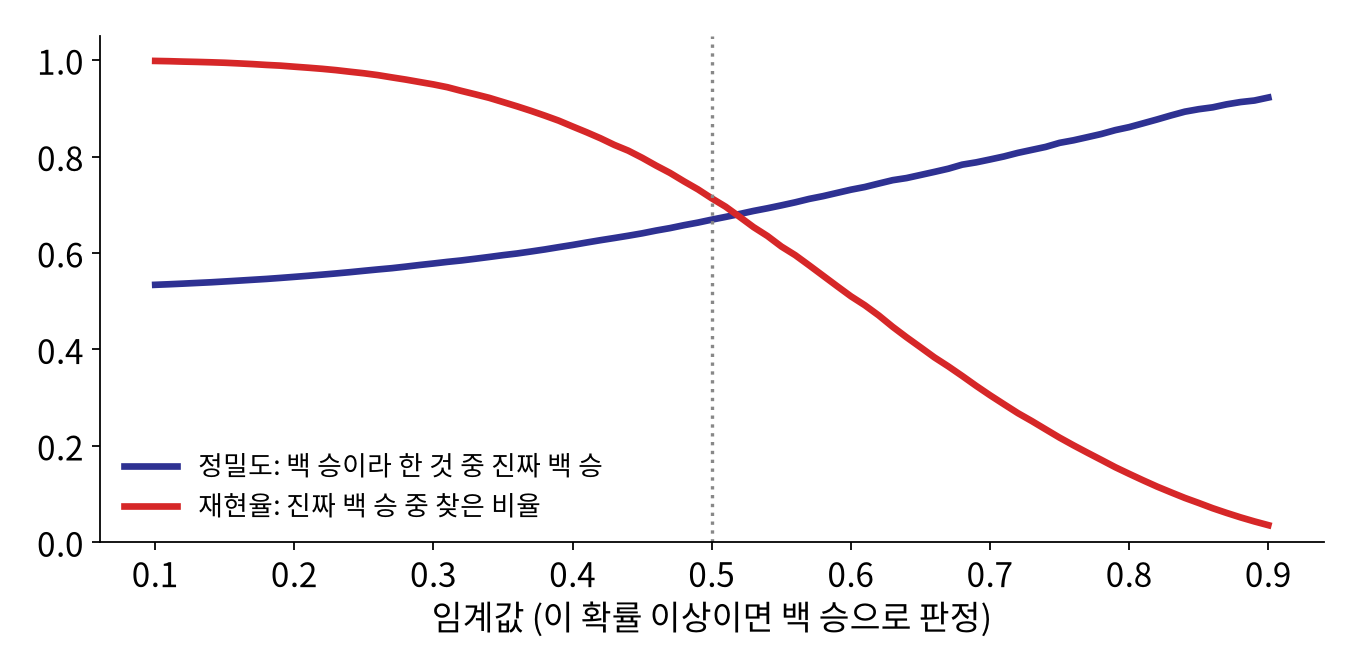
\includegraphics[width=0.6\linewidth]{chess_threshold.png}\par\vskip0.2em
{\large 임계값을 올리면 \kb{정밀도} $\uparrow$ \kq{재현율} $\downarrow$ \quad 무엇을 놓치면 더 곤란한지로 정한다}\\[0.2em]
{\small 0.5 에서: 백 승이라 한 판의 67\% 가 진짜 백 승, 진짜 백 승 61,926판 중 71\% 를 찾았다}
\vfill
\note{확률 0.5 이상을 백 승이라고 하는 건 하나의 선택일 뿐입니다. 임계값을 올리면 확실한 판만 백 승이라고 하니까, 백 승이라고 한 것 중 진짜 백 승 비율인 정밀도는 오르고, 진짜 백 승 중 찾아낸 비율인 재현율은 내려갑니다. 0.5에서는 정밀도 67퍼센트, 재현율 71퍼센트입니다. 레이팅 차이 하나만 보니 정확도에 한계가 있죠. 어떤 일에 쓰느냐에 따라, 헛짚는 게 더 곤란하면 임계값을 높이고, 놓치는 게 더 곤란하면 낮춥니다. 임계값을 모두 훑어서 정밀도와 재현율을 그린 것이 다음 주에 배울 PR 곡선입니다.}
\end{frame}

\section{연습}
% --- 문제풀이
\begin{frame}{문제풀이}
\vfill
\begin{enumerate}
\item $\sigma(0)$ 은? $\sigma(z) = 0.9$ 이면 $z$ 는? \; ($\ln 9 \approx 2.2$)\vskip0.7em
\item 모델 $\hat y = \sigma(-6 + 1.5\,x)$. (a) 결정 경계 $x$ 는? \; (b) $x = 4$ 일 때 $\hat y$ 는?\vskip0.7em
\item $w_1 = 0.7$ 이면 $x$ 가 1 늘 때 오즈는 몇 배? \; ($e^{0.7} \approx 2.0$)\vskip0.7em
\item 정답 $y = 1$, 예측 $\hat y = 0.8$, 입력 $x = 3$. 이 데이터 하나의 $\partial J / \partial w_1$ 은? \pref{grad}
\end{enumerate}
\vfill
\note{1번 답. 시그모이드 0은 0.5입니다. 시그모이드 z가 0.9이면 오즈가 0.9 나누기 0.1, 9이니까 z는 ln 9, 약 2.2입니다. 2번 답. 경계는 z가 0인 곳, 마이너스 6 더하기 1.5 x가 0이니 x는 4입니다. 그래서 x가 4이면 정확히 경계 위라서 확률은 0.5입니다. 3번 답. e의 0.7제곱, 약 2배입니다. 4번 답. 오차 와이햇 빼기 y는 마이너스 0.2, 여기에 x 3을 곱해서 마이너스 0.6입니다. 기울기가 음수이니 w1을 키우는 쪽으로 갑니다.}
\end{frame}

% --- 실습
\begin{frame}[fragile]{실습}
\vfill
\centering\begin{tabular}{rl}
\large 1 & 선형회귀 코드에서 한 줄 바꿔 로지스틱회귀 구현 (``200점 높으면 74\%'' 재현, Elo 와 비교)\\[0.5em]
\large 2 & 백 레이팅 · 흑 레이팅을 따로 넣고 100점당 오즈 배수 읽기\\[0.5em]
\large 3 & 임계값을 바꿔 정밀도 · 재현율 보기, PR 곡선과 PR-AUC
\end{tabular}\vskip1em
lichess 체스 117,003판 (2013년 1월, CC0) \\[0.4em]\href{https://colab.research.google.com/github/SuminHan/book-ml/blob/main/slides/v2_cs/ml1/week02/2_logistic_regression/lab/logistic_regression.ipynb}{\textcolor{ksagolddk}{▶ Colab에서 실습 노트북 열기}}
\vfill
\note{실습은 세 부분입니다. 첫째, 지난 시간의 선형회귀 경사하강법 코드에서 예측 줄 하나를 시그모이드로 바꿔 로지스틱회귀를 만들고, 오늘 본 체스 11만 판으로 백이 200점 높으면 74퍼센트라는 숫자를 직접 재현합니다. Elo 공식 곡선과도 겹쳐 봅니다. 둘째, 레이팅 차이 대신 백 레이팅과 흑 레이팅을 따로 넣고, 100점당 오즈 배수를 읽어 봅니다. 두 계수 크기가 거의 같아서 결국 차이만 중요하다는 것도 확인합니다. 셋째, 임계값을 바꿔 가며 정밀도와 재현율이 어떻게 바뀌는지 보고 PR 곡선을 그립니다.}
\end{frame}

\section{정리}
% --- 정리
\begin{frame}{정리}
\vfill
\centering\large\begin{tabular}{l}
모델 \quad $\hat y = \sigma(w_0 + w_1 x)$ = 1일 확률\\[0.5em]
결정 경계 \quad $z = 0$ (특징이 여럿이어도 곧은 경계)\\[0.5em]
해석 \quad $x$ 가 1 늘면 오즈가 $e^{w_1}$ 배\\[0.5em]
학습 \quad 교차 엔트로피 + 경사하강법 (기울기는 선형회귀와 같은 모양)\\[0.5em]
판정 \quad 임계값은 정밀도 · 재현율을 보고 정한다\\[0.5em]
체스 12만 판 \quad 백이 200점 높으면 74\%, 100점마다 오즈 1.6배, Elo 도 로지스틱
\end{tabular}
\vfill
\note{정리합니다. 로지스틱회귀는 직선에 시그모이드를 씌워 1일 확률을 내는 모델입니다. 결정 경계는 z가 0인 곳이고, 특징이 여럿이어도 곧은 경계입니다. w1은 x가 1 늘 때 오즈가 e의 w1제곱 배가 된다고 읽습니다. 학습은 교차 엔트로피와 경사하강법으로 하고, 기울기는 선형회귀와 같은 모양입니다. 마지막으로 0.5라는 임계값은 정밀도와 재현율을 보고 문제에 맞게 정합니다.}
\end{frame}
\end{document}
